%!TEX TS-program = xelatex

% -- Document Class -----------------------------------------------------------

\documentclass[a4paper, 12pt]{article}

% -- Packages -----------------------------------------------------------------

% Language
\usepackage{polyglossia}
    \setmainlanguage{english}
    \setotherlanguage{german}
% Context sensitive quotation
\usepackage{csquotes}
% Customize enumerations
\usepackage{enumitem}
% Extend options for positioning floats
\usepackage{float}
% Support highlighting of certain parts of the text
\usepackage{framed}
% Support spaces in filenames
\usepackage{grffile}
% Tools for mathematical typesetting
\usepackage{mathtools}
% Headers & Footers
\usepackage[automark, nouppercase]{scrpage2}
% Emphasize text
\usepackage{soul}
% To change the format of titles
\usepackage{titlesec}
% Support for unicode math fonts
\usepackage{unicode-math}
% Extended color support
\usepackage[x11names]{xcolor}
% Extras for XƎTEX
\usepackage{xltxtra}
% Hyperlinks and pdf properties
\usepackage{hyperref}

% -- Color Definitions --------------------------------------------------------

% Background color for syntax highlighting
\definecolor{bgcolor}{rgb}      {1,     1,      1}

% Custom color definitions
\definecolor{aqua}{rgb}         {0,     0.56,   1}
\definecolor{bluegray}{rgb}     {0.22,  0.46,   0.84}
\definecolor{grape}{rgb}        {0.56,  0,      1}
\definecolor{lightgray}{rgb}	{0.94,	0.94,	0.94}
\definecolor{orchid}{rgb}       {0.41,  0.13,   0.55}
\definecolor{orange}{rgb}       {1,     0.54,   0}
\definecolor{silver}{rgb}       {0.57,  0.57,   0.57}
\definecolor{turquoise}{rgb}    {0,     0.86,   0.84}

% -- Macros -------------------------------------------------------------------

\newcommand{\Title}{Exercises}
\newcommand{\TitleDescription}{Computer Aided Verification}
\newcommand{\Version}{1}
\newcommand{\Subject}
    {Solutions for the exercises of the course Computer Aided Verification}
\newcommand{\KeyWords}{BDD, Kripke structure}
\newcommand{\LeftFooter}{\Title~—~\TitleDescription}

\newcommand{\AuthorOne}{René Schwaiger}
\newcommand{\MailOne}{\href{mailto:sanssecours@f-m.fm}{sanssecours@f-m.fm}}

% Syntax highlighting definitions
% Text
\newcommand{\hlstd}[1]{\textcolor{black}{#1}}
% Numbers
\newcommand{\hlnum}[1]{\textcolor{DarkOrchid4}{#1}}
\newcommand{\hlesc}[1]{\textcolor[rgb]{1,0,1}{#1}}
% Strings
\newcommand{\hlstr}[1]{\textcolor{SeaGreen3}{#1}}
\newcommand{\hlpps}[1]{\textcolor[rgb]{0.51,0.51,0}{#1}}
% Comments
\newcommand{\hlslc}[1]{\textcolor{aqua}{#1}}
\newcommand{\hlcom}[1]{\textcolor{aqua}{#1}}
\newcommand{\hlppc}[1]{\textcolor[rgb]{0,0.51,0}{#1}}
\newcommand{\hlopt}[1]{\textcolor[rgb]{0,0,0}{#1}}
\newcommand{\hllin}[1]{\textcolor[rgb]{0.33,0.33,0.33}{#1}}
% Keywords
\newcommand{\hlkwa}[1]{\textcolor{DodgerBlue3}{#1}}
\newcommand{\hlkwb}[1]{\textcolor[rgb]{0,0.34,0.68}{#1}}
\newcommand{\hlkwc}[1]{\textcolor{DarkOrchid4}{#1}}
% Functions
\newcommand{\hlkwd}[1]{\textcolor{orange}{#1}}

\newcommand{\codeinput}[1]
{
    {\color{lightgray}\hrule}\vskip 0.3 cm
    {\fontsize{9pt}{11pt}\input{Code/#1}}
    \vskip 0.3 cm{\color{lightgray}\hrule}
}

\newcommand{\code}[1]
{
    \hl{\texttt{#1}}
}

% -- Document Properties ------------------------------------------------------

% Background color for highlighted text
\sethlcolor{lightgray}

% No indentation after paragraphs
\setlength\parindent{0cm}

% Hyperref properties
\hypersetup
{
    pdftitle    = {\Title},
    pdfsubject  = {\Subject},
    pdfauthor   = {\AuthorOne},
    pdfkeywords = {\KeyWords},
    colorlinks  = true,
    linkcolor   = black,
    anchorcolor = black,
    citecolor   = silver,
    urlcolor    = orange
}

% -- Fonts --------------------------------------------------------------------

% Use same size for numbers and other text
\defaultfontfeatures{Numbers=Lining}

% Set fonts for document
\setmainfont[Mapping=tex-text]{Avenir Next}
\setsansfont[Mapping=tex-text]{Ubuntu}
\setmonofont[Scale=MatchLowercase]{Menlo}
\setmathfont{Asana-Math.otf}
\setmathfont[range=\mathtt, Scale=MatchLowercase]{Menlo}

% Define font styles
\newfontfamily\Zapfino{Zapfino}

% -- Header And Footers -------------------------------------------------------

% Use normal font instead of italic font for head
\renewcommand{\headfont}{\normalfont}

% Set headers and footers
\ihead{\headmark}
\ohead{}
\ifoot{\LeftFooter}
\ofoot{\thepage}

% Set height of head
\setlength{\headheight}{1.8\baselineskip}

% Set thickness of separation line in header, footer
\setheadsepline{0.5pt}
\setfootsepline{0.5pt}

% -- Titlepage ----------------------------------------------------------------

\pagestyle{empty}
\begin{document}

\begin{titlepage}
    \begin{center}
        % Title and title-description
        {\Huge\Zapfino\Title}
        \vskip 0.5cm
        {\color{aqua}\hrule}
        \vskip 0.5cm
        {\Large\textit\TitleDescription}
        \vskip 14cm
    \end{center}

    % Date and version number
    \begin{leftbar}
        \begin{tabular}{ll}
            \textbf{Author}  & \AuthorOne\\
            \textbf{Mail}    & \MailOne\\
            \textbf{Version} & \Version\\
            \textbf{Date}    & \today
        \end{tabular}
    \end{leftbar}

\end{titlepage}


% -- Table of Contents --------------------------------------------------------

% Set section format for table of contents
\titleformat{\section}{\sffamily\bfseries}{}{0pt}{}[{\color{aqua}\hrule}]

% Set separation of dots between name of section and page number to such a high
% value that there will be no points in the table of contents
\makeatletter \renewcommand{\@dotsep}{10000} \makeatother
% Use blank header and footer
\pagestyle{empty}
% Start on new page
\newpage
% The table of contents starts at the second page
\setcounter{page}{2}
% Set table of contents
\tableofcontents

% -- Section & Paragraph Style ------------------------------------------------

% Set format for section
\titleformat{\section}
    {\large\sffamily\bfseries}  % Large, bold, sans serif font for section
    {}                          % No format applied to whole title
    {0pt}                       % No separation between label and title
    {\thesection~·~}            % Start with section number
    [{\color{aqua}\hrule}]      % Underline with blue ruler

% Set format for other sections and paragraphs
% Color = orchid, Font = bold, sans serif
\titleformat*{\subsection}{\color{orchid}\sffamily\bfseries}
\titleformat*{\subsubsection}{\color{orchid}\sffamily\bfseries}
\titleformat*{\paragraph}{\color{orchid}\sffamily\bfseries}
\titleformat*{\subparagraph}{\color{orchid}\sffamily\bfseries}

% -- Page Style ---------------------------------------------------------------

% Start with text on a new page
\newpage
% Display headers and footers
\pagestyle{scrheadings}

% -- Text ---------------------------------------------------------------------

\section{Binary Decision Diagrams}

\subsection{Exercise 1}

Give a linear time algorithm for BDD isomorphism as defined on page 9.

\subsubsection{Solution}

The following code assumes the existence of the functions:

\begin{description}[style=multiline, leftmargin=3.5cm]
    \item[\texttt{is\_terminal(v)}] Returns \texttt{True} if \texttt{v} is a terminal vertex and \texttt{False} otherwise
\end{description}

\paragraph{Nonterminal Vertices}

\begin{description}[style=multiline, leftmargin=3.5cm]
    \item [\texttt{var(v)}] Returns the variable of a BDD vertex.
    \item [\texttt{low(v)}] Returns the “low” successor of the BDD vertex (v is set to 0)
    \item [\texttt{high(v)}] Returns the “high” successor of the BDD vertex (v is set to 1)
\end{description}

\paragraph{Terminal Vertices}

\begin{description}[style=multiline, leftmargin=3.5cm]
    \item[\texttt{high(v)}] Returns the value of v (Either 0 or 1)
\end{description}

\codeinput{isomorphic}

\subsection{Exercise 2}

Show that the three operations on page 12 commute.

\subsection{Exercise 3}

Describe a size-efficient BDD for the relation “a<b” for n-bit integer numbers.

\subsubsection{Solution}

We assume that:

\begin{itemize}
    \item $a$ has the form $a_na_{n-1}…a_0$, where $a_n$ ist the most significant bit.
    \item $b$ is encoded in the same way as $a$.
    \item Both $a$ and $b$ are positive numbers.
\end{itemize}

Figure~\ref{fig:Figures_OBDD_Smaller} shows the BDD that encodes the boolean operation “a<b”.

\begin{figure}[h]
  \centering
    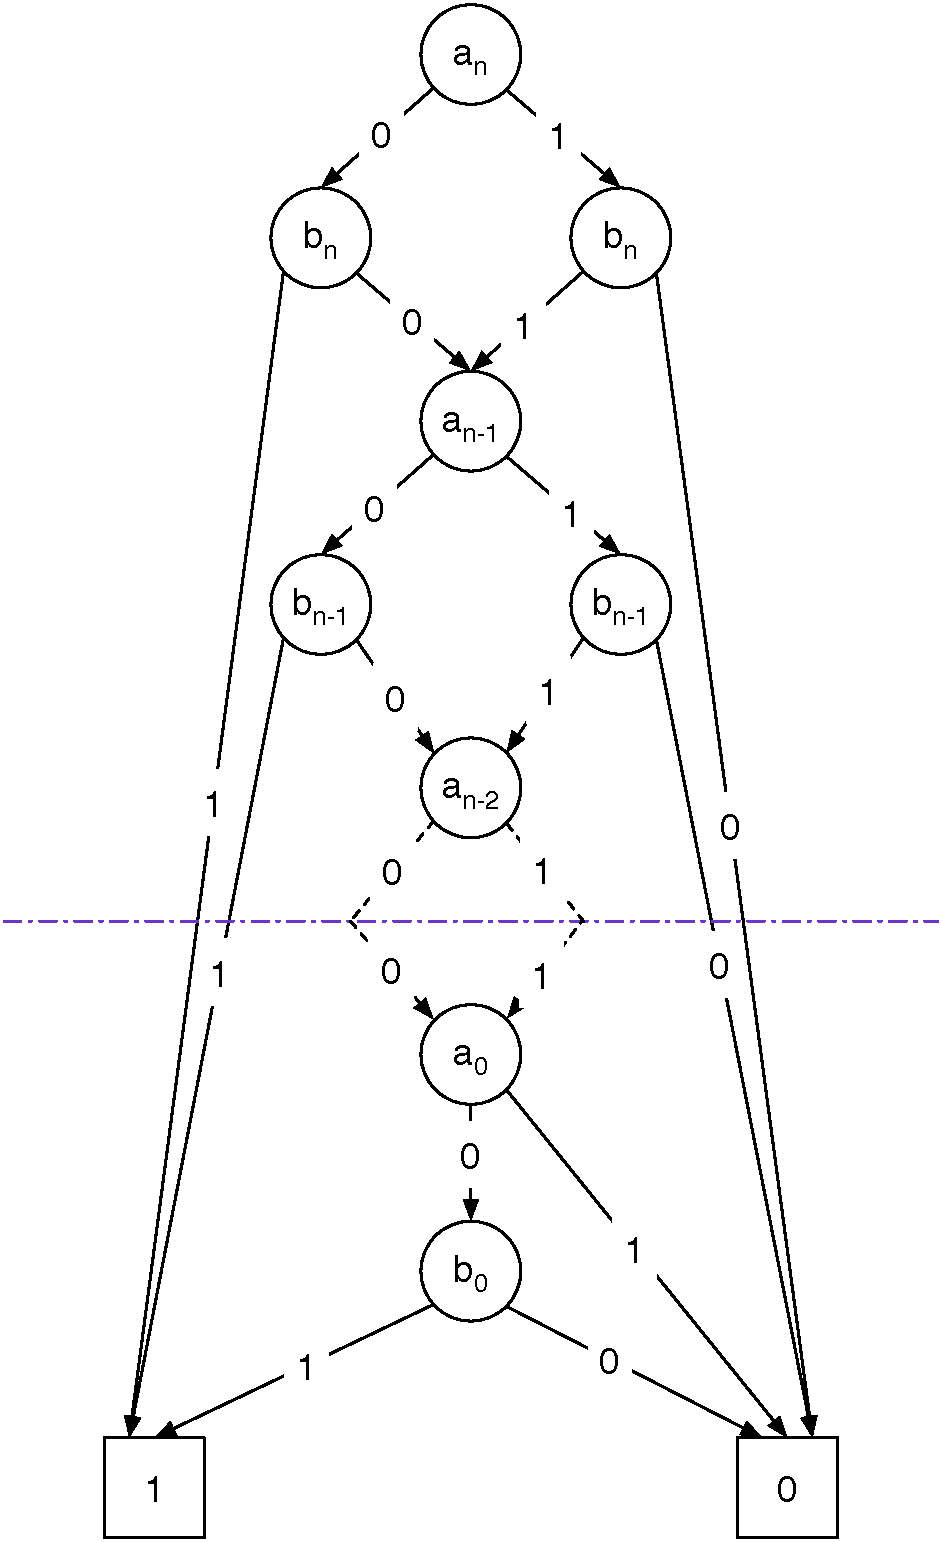
\includegraphics[width=.54\textwidth]{Figures/OBDD Smaller.pdf}
  \caption{An OBBD for the operation “a<b”}
  \label{fig:Figures_OBDD_Smaller}
\end{figure}

\subsection{Exercise 4}

Describe an algorithm which transforms a Boolean formula into an equivalent Binary decision diagram

\section{Temporal Logic}

\subsection{Exercise 5}

Prove the equivalence for A(f U g) on page 16.

\subsection{Exercise 6}

Show the following lemma: Let M and N be two Kripke structures such that the transition relation of M is a superset of the transition relation of N. If an LTL property f holds on M, then f also holds on N.

\subsection{Exercise 7}

Show AFG p is not logically equivalent to AFAG. Which of the two formulas implies the other one?

\subsection{Exercise 8}

Show that all LTL properties have counterexamples which are either finite paths or finite paths which lead to a loop.

\subsection{Exercise 9}

Give an LTL specification and a Kripke structure where the smallest counterexample is larger than the number of states in the Kripke structure.

\subsection{Exercise 10}

Show how you can use SMV to solve the Rubik’s cube.

\section{Questions to Test Your Understanding}

Are the following statements correct/false? Why?

\begin{enumerate}[label=(\alph*)]
    \item CTL is contained in LTL
    \item LTL is contained in CTL*
    \item Every CTL formula is equivalent to a formula containing only E, but no A
    \item Every LTL formula is equivalent to a negation-free formula containing only A, but no E
    \item For each Boolean function f over n variables, there exists an order on the variables such that the BDD for f has size linear in n.
    \item Every BDD can be translated into an equivalent Boolean formula.
    \item On a Kripke structure M, the size of a counterexample is bounded by the number of states in M, multiplied by the size of the specification.
    \item Bounded model checking can be used to find the smallest counterexample.
    \item In SMV, each BDD node corresponds to a state in the Kripke structure.
    \item In SMV, BDDs are used as specification language.
\end{enumerate}

\end{document}
